\chapter{Durchführung}
\label{chap:Durchfuehrung}

In der bereits hergeleiteten Theorie wird der Lösungsweg für das beschrieben Problem vorgestellt. Mit dem zur Verfügung gestelltem Skript, das auf dieser Theorie basiert wird nun die Parameterstudie durchgeführt. Um relevante Ergebnisse zu erlangen, müssen zuerst weitere Gleichungen in das Skript eingearbeitet werden.\\
In dem Skript wird eine Konstante $c$ als Vorfaktor für die Kraftberechnung aus dem Punktkontakt verwendet. Um die Berechnungsmöglichkeiten zu erweitern, wird $c$ nun durch eine Gleichung der Hertz'schen Pressung ersetzt, die wie folgt Hergeleitet wird:\\
Die Gleichung für die Hertz'sche Pressung eines Kugel-Kugel-Punktkontaktes lautet wie in Gleichung~\ref{form:ZvonP}

\begin{equation}
	\label{form:ZvonP}
	z(P) = \left[ \frac{9 P^{2} (1 - \nu^{2})^{2}}{2 E^{2}} \cdot \left( \frac{1}{2 r_{1}} + \frac{1}{2 r_{2}} \right) \right]^{\frac{1}{3}}
\end{equation}

Da einer der beiden Körper eine Platte mit dem Radius $r_{p} = \infty$ ist, folgt durch einsetzen von $r_{p}$ und umstellen nach P:

\begin{equation}
	\label{form:PvonZ}
	P(z) = \sqrt{\frac{4 r_{g}}{9}} \cdot \frac{E}{(1 - \nu^{2})} \cdot z^{\frac{3}{2}}
\end{equation}
	
Hier ist $\frac{E}{(1 - \nu^{2})}$ der reduzierte E-Modul, welcher durch Gleichung~\ref{form:redE} beschrieben wird.

\begin{equation}
	\label{form:redE}
	\frac{E}{(1 - \nu^{2})} = \left( \frac{(1 - \nu_{p}^{2})}{E_{p}} + \frac{(1 - \nu_{g}^{2})}{E_{g}} \right)^{-1}
\end{equation} 

Nun wird $c$ als Vorfaktor von $z^{\frac{3}{2}}$ in Gleichung~\ref{form:PvonZ} definiert, sodass folgt:

\begin{equation}
	\label{form:c}
	c = \sqrt{\frac{4 r_{g}}{9}} \cdot \frac{E}{(1 - \nu^{2})}
\end{equation}

Im Skript wurden Gleichungen~\ref{form:redE} und~\ref{form:c} unter den Konstanten implementiert und die einstellbaren Parameter der Platte und der Impaktor respektive um $E_{p}$ und $\nu_{p}$, bzw. $E_{g}$ und $\nu_{g}$ erweitert.\\

\section{Vorgehen und Vorbereitung}

Insgesamt wird das Problem durch die einstellbaren Parameter in Tabelle~\ref{tab:VariablenderStudie} beschrieben. In Anlehnung an \cite{Olsson.2000} wird das Massenverhältnis $MR$ als einer der signifikanten Parameter gewählt. Davon ausgehend werden dann die anderen Parameter einzeln variiert und die Ergebnisse grafisch ausgewertet. 

\begin{table}[H]
	\begin{center}
		\caption{Variablen der Parameterstudie}
		\label{tab:VariablenderStudie}
		\begin{tabular}{l|c}
			\textbf{Variable} & \textbf{Bedeutung}\\
			\hline
			$a,b,h$ & Plattenmaße in [cm]\\
			$r_{g}$ & Impaktorradius in [cm]\\
			$v_{0}$ & Auftreffgeschwindigkeit [cm/s]\\
			$MR$ & Massenverhältnis $\hat{=}$ $\frac{Impaktormasse}{Plattenmasse}$\\
			$\xi,\eta$ & Auftreffstelle des Impaktors\\
			$x,y$ & Auswertungsstelle\\		
		\end{tabular}
	\end{center}
\end{table}

\subsection{Auswertungskriterien und Annahmen}

Als Auswertungskriterien werden die Anzahl der einzelnen Schläge und der maximal auftretenden Kraft zusammen mit der Auslenkung der Platte gewählt. \\
Für die Studie werden folgende übergreifende Annahmen getroffen: 

\begin{enumerate}
	\item{Die Platte und der Impaktor sind isotrop, mit konstanten Stoffwerten}
	\item{Die Platte und der Impaktor sind aus identischem Material, mit gleichem E-Modul und Poissonzahl $\nu$}
\end{enumerate}

\subsubsection{Anzahl der Schläge}

Als Schlag wird hier ein Kraftverlauf bezeichnet, bei dem die Kraft $P_{i}$ zwischen den Schlägen auf Null fällt, nach der Bedingung in Gleichung~\ref{form:Schlagauftreten}:

\begin{equation} 
	\label{form:Schlagauftreten}
	F_{i-1} > 0 \; \wedge \; F_{i} = 0 
\end{equation}

Da im zeitlichen Verlauf auch nach dem ersten Auftreffen noch Schläge auftreten können, wird die Schrittanzahl auf $i = 1000$ gesetzt um signifikante Ergebnisse zu erlangen. 

\subsubsection{Maximale Kraft}

Die maximale Kraft $P_{max}$ wird direkt aus der Versuchsreihe ausgelesen und in Abhängigkeit des Massenverhältnisses dargestellt.

\subsubsection{Maximale Auslenkung der Platte}
Analog zur maximalen Kraft, wird die maximale Auslenkung $w_{max}$ direkt ausgelesen und in Abhängigkeit von $MR$ dargestellt.

\subsection{Programmanpassungen}

Um die große Mengen an Daten aus den Versuchsreihen auffassen zu können, werden zwei Schleifen implementiert, die jeweils über den berücksichtigten Parameter und das Massenverhältnis iterieren. Diese geben die Daten dann in der Form von $.txt$ Dateien aus, die über Gnuplot ((ANHANG GNUPLOT Einstellen mit Skripten und ref)) zu 2-D, bzw. 3-D Grafiken verarbeitet werden.\\
Außerdem wird eine Funktion $compute()$ definiert, mit der man die betrachteten Parameter direkt variieren kann ohne den Quellcode zu verändern. 

\section{Parameterstudie}

Für die Parameterstudie wurde folgender Fall aus Ausgangspunkt gewählt: 

\begin{table}[H]
	\begin{center}
		\caption{Ausgangsfall Parameterstudie}
		\label{tab:Ausgang}
		\begin{tabular}{l|c}
			\textbf{Variable} & \textbf{Wert}\\
			\hline
			$a$ & 50.0 [cm]\\
			$b$ & 50.0 [cm]\\
			$h$ & 1.0 [cm]\\
			$r_{g}$ & 1.0 [cm]\\
			$v_{0}$ & 500.0 [cm/s]\\
			$\xi,\eta$ & 25.0 [cm]\\
			$x,y$ & 25.0 [cm]\\ 		
		\end{tabular}
	\end{center}
\end{table}

$MR$ wird hier bewusst ausgelassen, da bei jedem Parameter über das Massenverhältnis iteriert wird und dadurch kein Anfangswert, sondern eine Menge, benötigt wird. Die Menge der $MR$ ist nach Gleichung~\ref{form:MR}:

\begin{equation}
	\label{form:MR}
	0.01 \leq MR \leq 2.50 \; , \;\; \mbox{Schrittweite:} \; \Delta MR = 0.01
\end{equation}

Die Stoffparameter sind im Rahmen der Studie konstant und in Tabelle~\ref{tab:Stoff} definiert.

\begin{table}[H]
	\begin{center}
		\caption{Stoffparameter: Kugel und Platte}
		\label{tab:Stoff}
		\begin{tabular}{l|c}
			\textbf{Variable} & \textbf{Wert}\\
			\hline
			$E_{p}$ & $2.2 \cdot 1e06$ [$kg/cm^2$]\\
			$\nu_{p}$ & 0.3 [-]\\
			$\rho_{p}$ & 0.00796 [$kg/cm^{3}$]\\
			\hline
			$E_{g}$ &  $2.2 \cdot 1e06$ [$kg/cm^2$]\\
			$\nu_{g}$ & 0.3 [-]\\		
		\end{tabular}
	\end{center}
\end{table}

\subsection{Höhe der Platte}

Als erster Parameter wird die Höhe nach Gleichung~\ref{form:DeltaH} variiert.

\begin{equation}
	\label{form:DeltaH}
	0.5 [cm] \leq h \leq 2.5 [cm], \; \; \mbox{Schrittweite:} \; \Delta h = 0.1 [cm]
\end{equation}

Wenn man die Höhe, das Massenverhältnis und die Anzahl der Schläge aufträgt, ergibt sich Abbildung~\ref{fig:Hoehe}. 

\begin{figure}[H]
	\begin{center}
		\begin{overpic}[width=\linewidth]{pictures/gnuplot/3d/Hoehe/production/Hoehe.eps}
			\put(45,4){Höhe [cm]}
			\put(18,30){\rotatebox{90}{Mr [-]}}
			\put(83,60){Aufschläge [-]}
		\end{overpic}
	\label{fig:Hoehe}
	\caption{Höhe, MR und Anzahl der Aufschläge}
	\end{center}
\end{figure}

Man kann direkt ablesen, dass mehrere Aufschläge vermehrt im unteren Höhenbereich auftreten. Dies ist direkt auf die Steifigkeit der Platte zurückzuführen. Bei größerer Plattendicke ist die Steifigkeit der Platte größer und die Kugel prallt ab, ohne vermehrt aufzutreffen.

\begin{figure}[H]
	\begin{center}
		\begin{overpic}[width=\linewidth]{pictures/gnuplot/3d/Hoehe/production/HoeheAuslenkung.eps}
			\put(72,11){Höhe [cm]}
			\put(16,11){MR [-]}
			\put(1,55){Auslenkung [cm]}
		\end{overpic}
	\label{fig:HoeheAuslenkung}
	\caption{Höhe, MR und Auslenkung}
	\end{center}
\end{figure}

\begin{figure}[H]
	\begin{center}
		\begin{overpic}[width=\linewidth]{pictures/gnuplot/3d/Hoehe/production/HoeheKraft.eps}
			\put(82,15){Höhe [cm]}
			\put(40,9){MR [-]}
			\put(9,50){Kraft [N]}
		\end{overpic}
	\label{fig:HoeheKraft}
	\caption{Höhe, MR und Kraft}
	\end{center}
\end{figure}

\subsection{Geschwindigkeit des Impaktors}

\begin{figure}[H]
	\begin{center}
		\begin{overpic}[width=\linewidth]{pictures/gnuplot/3d/Speed/production/Speed.eps}
			\put(40,4){Geschwindigkeit [cm/s]}
			\put(18,30){\rotatebox{90}{Mr [-]}}
			\put(83,60){Aufschläge [-]}
		\end{overpic}
		\label{fig:Speed}
		\caption{Geschwindigkeit, MR und Anzahl der Aufschläge}
	\end{center}
\end{figure}

\begin{figure}[H]
	\begin{center}
		\begin{overpic}[width=\linewidth]{pictures/gnuplot/3d/Speed/production/SpeedAuslenkung.eps}
			\put(57,8){Geschwindigkeit [cm/s]}
			\put(16,12){MR [-]}
			\put(1,56){Auslenkung [cm]}
		\end{overpic}
		\label{fig:SpeedAuslenkung}
		\caption{Geschwindigkeit, MR und Auslenkung}
	\end{center}
\end{figure}

\begin{figure}[H]
	\begin{center}
		\begin{overpic}[width=\linewidth]{pictures/gnuplot/3d/Speed/production/SpeedKraft.eps}
			\put(3,12){\begin{minipage}{\textwidth}Geschwindigkeit\\ in [cm/s]\end{minipage}}
			\put(58,8){MR [-]}
			\put(9,58){Kraft [N]}
		\end{overpic}
		\label{fig:SpeedKraft}
		\caption{Geschwindigkeit, MR und Kraft}
	\end{center}
\end{figure}


\subsection{Variation des Impaktortes}
Ebenfalls wird der Aufschlagsort des Impaktors verändert. Alle anderen Parameter aus Tabelle \ref{tab:Ausgang} und \ref{tab:Stoff} werden konstant gehalten. Um eine Verallgemeinerung zu gewährleisten, wurde der Aufschlagsort entdimensioniert. Hierfür wird statt $\xi$ und $\eta$, $\frac{\xi}{a}$ und $\frac{\eta}{b}$ verwendet. Da die Durchführung für eine quadratische Platte gemacht wurde, musste lediglich ein Achtel der gesamten Platte berechnet werden mit:

$$\left\lbrace  \left(\frac{\xi}{a},  \frac{\eta}{b}\right) \in \mathbb{R}^2 \vert \ 0.5 \le \frac{\xi}{a} \le 1 \ \land \ 0.5 \le \frac{\eta}{b} \le \frac{\xi}{a}  \right\rbrace $$


\begin{figure}[H]
	\begin{center}
		\begin{overpic}[width=\linewidth]{pictures/gnuplot/3d/xieta/production/XiEta.eps}
			\put(50,3){$\frac{\xi}{a}$ [-]}
			\put(83,60){Aufschläge [-]}
			\put(15,35){$\frac{\eta}{b}$ [-]}
		\end{overpic}
		\caption{Anzahl der Schläge durch Variation des Auftreffpunktes}
		\label{fig:xiEta}
	\end{center}
\end{figure}


Zunächst wird  der Einfluss der Position des Aufschlags auf die Anzahl der Schläge zwischen Platte und Kugel untersucht. 	
Es ist klar zu erkennen, dass ab einem gewissen Radius die Anzahl der Aufschläge konstant bei 1 ist. Dieser Radius liegt im Fall der quadratischen Platte unter den gegebenen Parametern bei ca. $0.23 \cdot a$. Da die Anzahl der Aufschläge in der Regel eine gewisse Abhängigkeit mit der Steifigkeit der Platte aufweist, ist es ersichtlich, dass die Platte am Rand eine erhöhte Steifigkeit aufweist und somit weniger Aufschläge hier auftreten.
Interessant ist jedoch die kreisförmige Ausbreiten der Grenze zwischen einem und zwei Aufschlägen. Ebenfalls ist die Unregelmäßigkeit der Anzahl der Aufschläge innerhalb dieses Kreises auffällig. Wenn die Plattensteifigkeit gering genug ist, konnte beobachtet werden, dass der erste Aufschlag die Geschwindigkeit der Kugel nur gering beeinflusst und durch eine höhere Relativgeschwindigkeit zwischen Platte und Kugel eine erhöhte Kraft beim zweiten Aufschlag beobachtet werden konnte.

\begin{figure}[H]
	\begin{center}
		\begin{overpic}[width=\linewidth]{pictures/gnuplot/3d/xieta/production/XiEtaAuslenkung.eps}
			\put(50,3){$\frac{\xi}{a}$ [-]}
			\put(86,60){max. Durchbiegung [cm]}
			\put(15,35){$\frac{\eta}{b}$ [-]}
		\end{overpic}
		\caption{maximale Durchbiegung durch Variation des Auftreffpunktes}
		\label{fig:xiEtaAuslenkung}
	\end{center}
\end{figure}

Für die maximale Durchbiegung in Abhängigkeit des Aufschlagortes, ergibt sich ein ähnliches Ergebnis wie für Anzahl der Aufschläge. Zunächst ist ebenfalls eine klare kreisförmige Grenze ersichtlich mit dem gleichen Radius wie in \ref{fig:xiEta}. Außerhalb dieses Kreises ist die maximale Durchbiegung einigermaßen konstant und nimmt kurz vor der Randfaser stark ab. In diesem Bereich befindet sich ebenfalls die maximale Durchbiegung bei $\frac{\xi}{a} = \frac{\eta}{b} = 0.75$. Hingegen ist die Durchbiegung im Plattenmittelpunkt gering im Vergleich zur maximalen Durchbiegung. Ebenfalls ist die maximale Durchbiegung innerhalb des Kreises, wie auch die Anzahl der Schläge, zufällig verteilt.


\begin{figure}[H]
	\begin{center}
		\begin{overpic}[width=\linewidth]{pictures/gnuplot/3d/xieta/production/XiEtaKraft.eps}
			\put(50,3){$\frac{\xi}{a}$ [-]}
			\put(90,60){max. Kraft [N]}
			\put(15,35){$\frac{\eta}{b}$ [-]}
		\end{overpic}
		\caption{maximale Kraft durch Variation des Auftreffpunktes}
		\label{fig:xiEtaKraft}
	\end{center}
\end{figure}
%\begin{figure}
%	\begin{center}
%		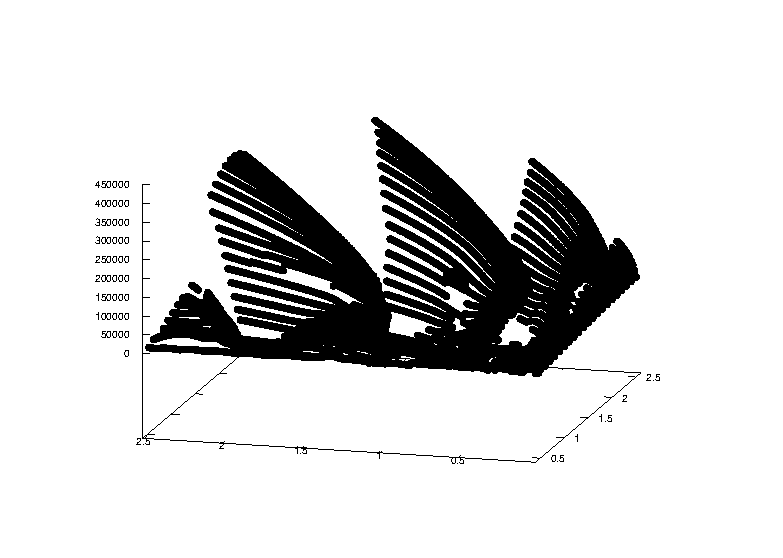
\includegraphics[width=\linewidth,angle=0]{pictures/gnuplot/3d/Hoehe/production/HoeheKraft.eps}
%	\end{center}	
%\end{figure}
	
	
 

	%Im zweiten Teil des Hauptteils folgt die Darstellung der eigenen Leistung. Aufbauend auf den im vorigen Kapitel erarbeiteten Grundlagen  wird nun der Lösungsweg aufgezeigt. Dabei wird das prinzipielle Vorgehen zum Erreichen der Zielsetzung unter Einbindung der verwendeten Hilfsmittel (Maschinen, Geräte, Programme etc. inklusive der verwendeten Einstellungen) aufgezeigt. Dabei müssen sämtliche verwendeten Daten ersichtlich sein, sodass es jederzeit möglich ist, die ermittelten Ergebnisse zu reproduzieren. Zum Schluss erfolgt unter Berücksichtigung der Randbedingungen eine kritische Analyse der Ergebnisse mit möglichen Unsicherheiten und Fehlern. Aus der Diskussion der Ergebnisse (z.B. Vergleich von Messwerten und theoretischen Vorhersagen), wird schließlich der Nutzen erörtert und mögliche weiterführende Fragestellungen werden erarbeitet.